\section{Solutions to exercises}
\label{sec:solutions}

\subsection{The optimal discriminator strategy}
\label{sec:opt_d_soln}

Our goal is to minimize
\begin{equation}
  J^{(D)}(\vtheta^{(D)}, \vtheta^{(G)}) = -\frac{1}{2} \E_{\vx \sim \pdata} \log D(\vx) - \frac{1}{2} \E_{\vz} \log \left(1 - D\left( G(z) \right) \right)
\end{equation}
in function space, specifying $D(\vx)$ directly.

We begin by assuming that both $\pdata$ and $\pmodel$ are nonzero everywhere.
If we do not make this assumption, then some points are never visited during training,
and have undefined behavior.

To minimize $J^{(D)}$ with respect to $D$, we can write down the functional derivatives with
respect to a single entry $D(\vx)$, and set them equal to zero:
\[
\frac{\delta} {\delta D(\vx)} J^{(D)} = 0.
\]
By solving this equation, we obtain
\[
D^*(\vx) = \frac{ \pdata(\vx) } {\pdata(\vx) + \pmodel(\vx) }.
\]

Estimating this ratio is the key approximation mechanism used by GANs.

The process is illustrated in \figref{fig:ratio}.

\begin{figure}
\centering
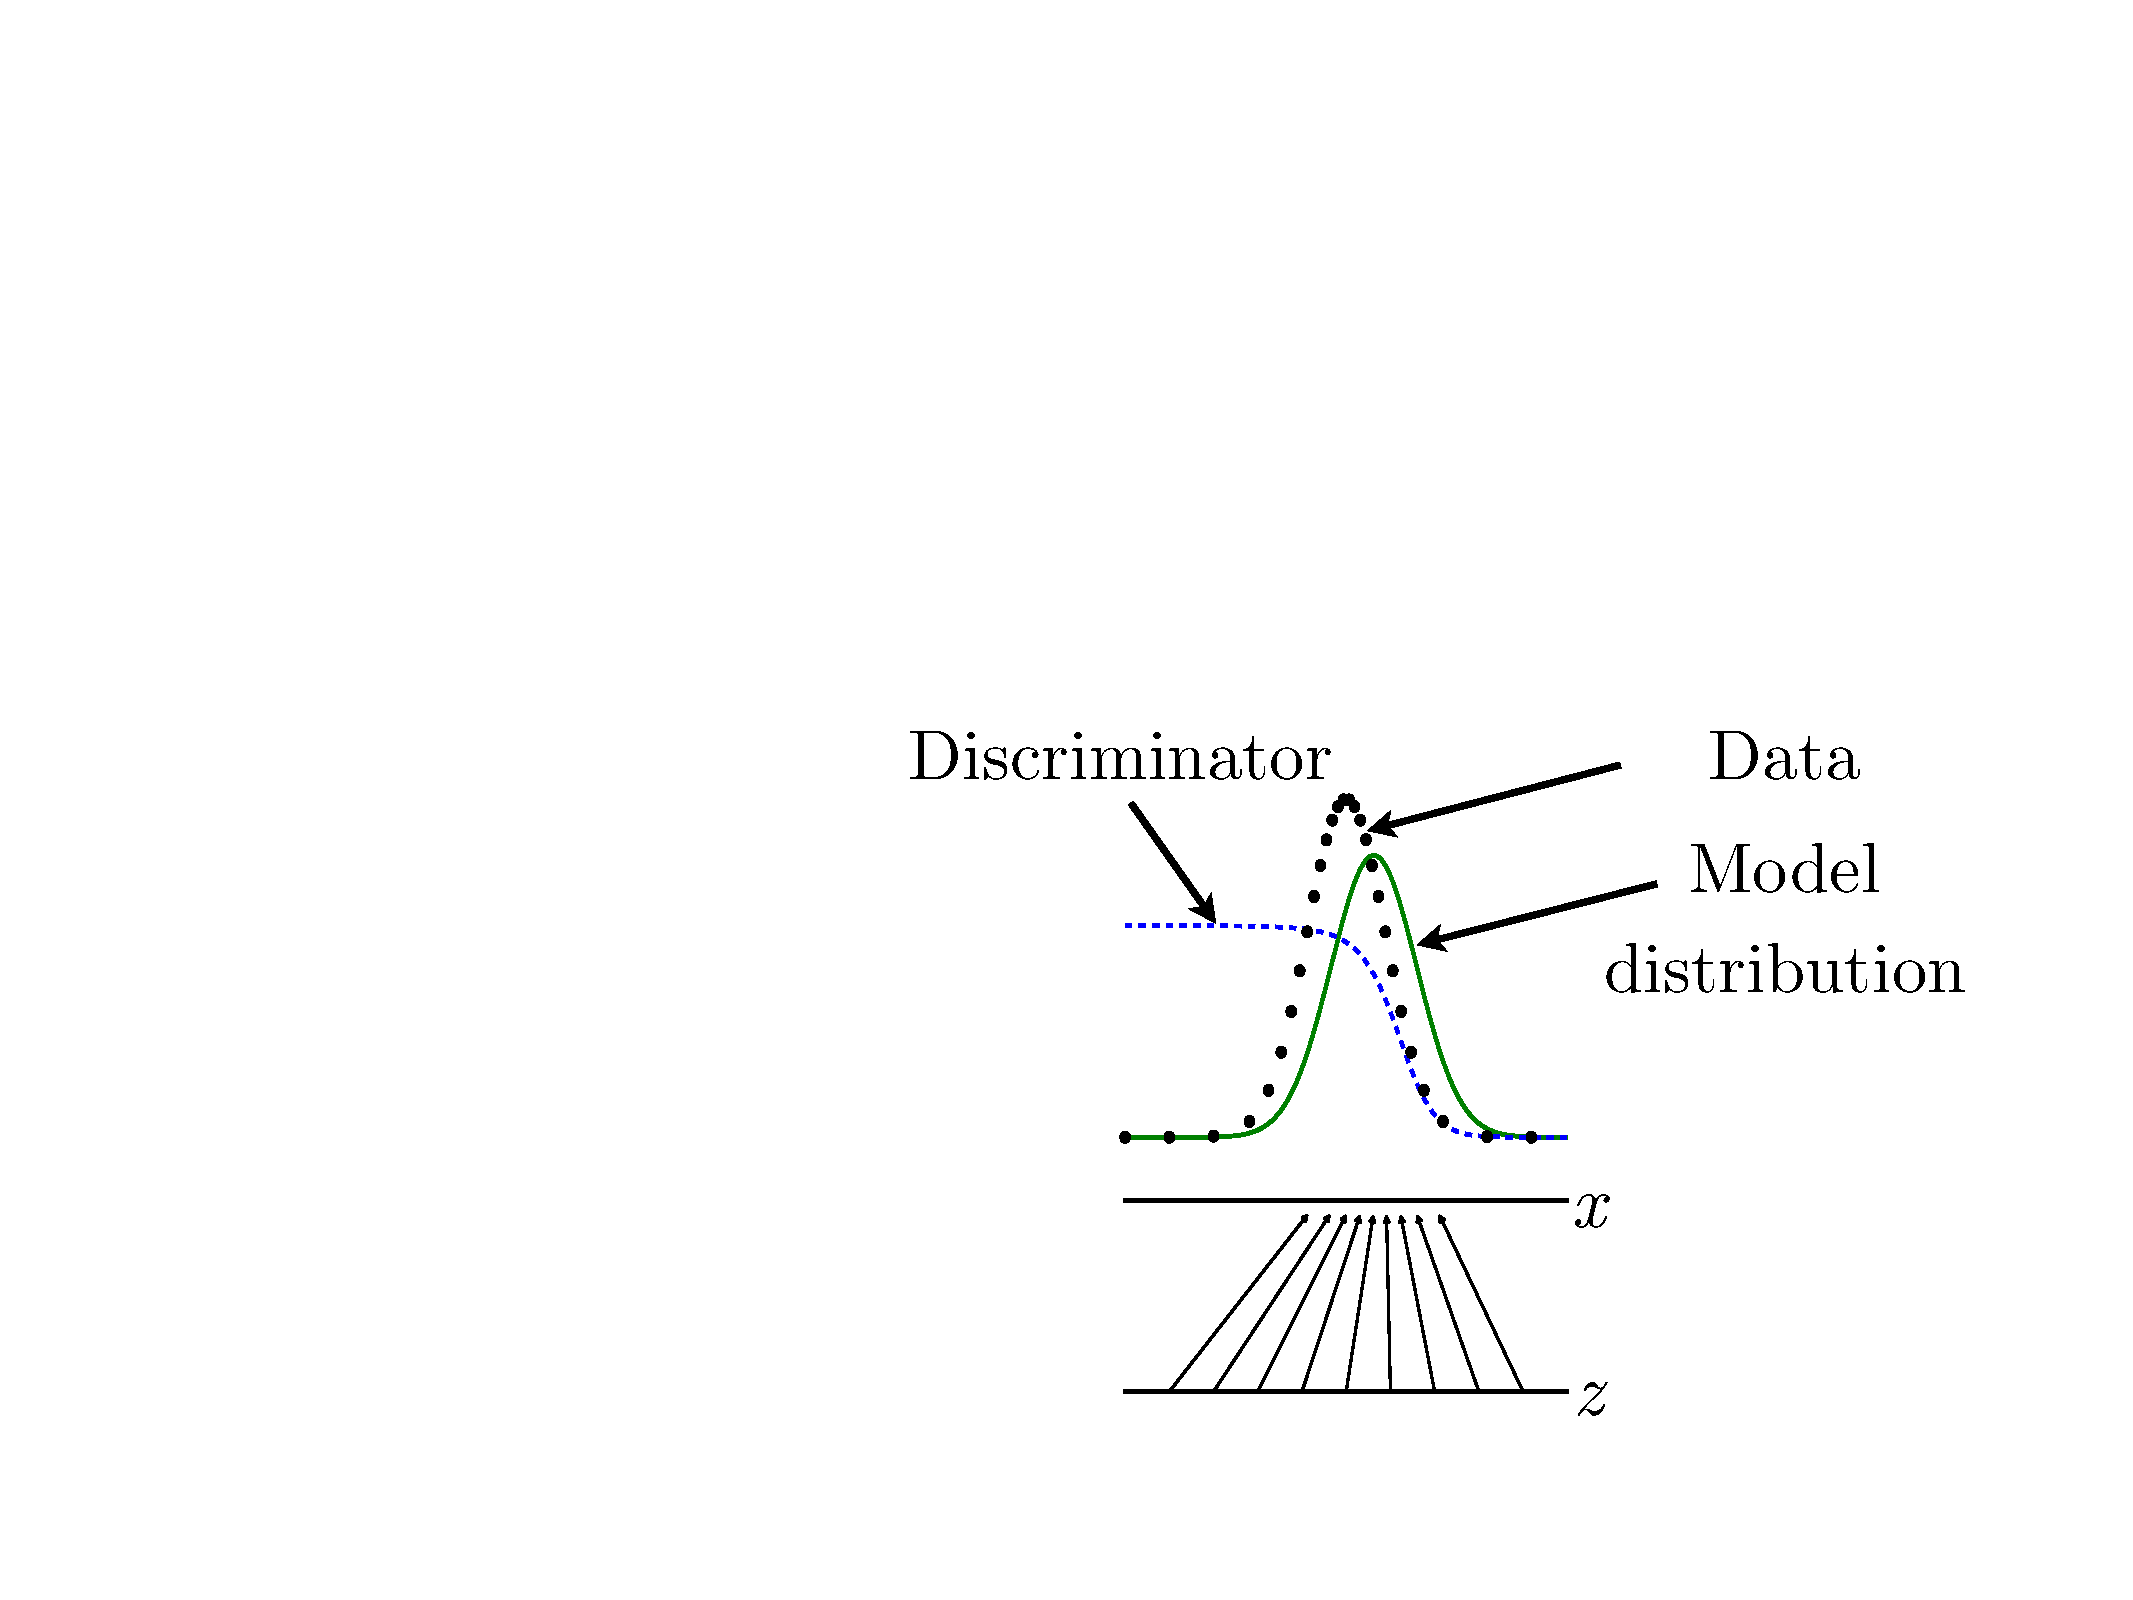
\includegraphics[width=\figwidth]{ratio}
\caption{
An illustration of how the discriminator estimates a ratio of
densities.
In this example, we assume that both $z$ and $x$ are one dimensional
for simplicity.
The mapping from $z$ to $x$ (shown by the black arrows) is non-uniform so that $\pmodel(x)$
(shown by the green curve) is
greater in places where $z$ values are brought together more densely.
The discriminator (dashed blue line) estimates the ratio between the data density (black dots)
and the sum of the data and model densities.
Wherever the output of the discriminator is large, the model density is too low, and wherever
the output of the discriminator is small, the model density is too high.
The generator can learn to produce a better model density by following the discriminator uphill;
each $G(z)$ value should move slightly in the direction that increases $D(G(z))$.
Figure reproduced from \citet{Goodfellow-et-al-NIPS2014-small}.
}
\label{fig:ratio}
\end{figure}


\subsection{TODO}

\subsection{Maximum likelihood in the GAN framework}
\label{sec:mle_soln}
TODO
